\documentclass[twoside,11pt,a4paper,openany]{book}
\usepackage[amsbb,subscriptcorrection,zswash,mtpcal,mtphrb]{mtpro2}
\usepackage[no-math,cm-default]{fontspec}
\usepackage{xunicode}
\usepackage{xgreek}
\defaultfontfeatures{Mapping=tex-text,Scale=MatchLowercase}
\def\xrwma{red!70!black}
\def\xrwmath{red!90!black}
\setmainfont[Mapping=tex-text,Numbers=Lining,Scale=1.0]{Minion Pro}
\newfontfamily\mpro{Minion Pro}
\usepackage{amsmath}
\usepackage[left=2.00cm, right=2.00cm, top=3.00cm, bottom=2.00cm]{geometry}
\usepackage{makeidx}
\usepackage{longtable}
\usepackage{etoolbox}
\makeatletter
\newif\ifLT@nocaption
\preto\longtable{\LT@nocaptiontrue}
\appto\endlongtable{%
\ifLT@nocaption
\addtocounter{table}{\m@ne}%
\fi}
\preto\LT@caption{%
\noalign{\global\LT@nocaptionfalse}}
\makeatother
\makeindex
\usepackage{tikz,pgfplots}
\usepackage{tkz-euclide,tkz-fct}
\usepackage{wrapfig}
\usetkzobj{all}
\usepackage{calc}
\usepackage{cleveref}
\usepackage[colorlinks=false, pdfborder={0 0 0}]{hyperref}
\usepackage[framemethod=TikZ]{mdframed}
\newcommand{\ypogrammisi}[1]{\underline{\smash{#1}}}
\usetikzlibrary{backgrounds}
\renewcommand{\thepart}{\arabic{part}}
\definecolor{steelblue}{cmyk}{.7,.278,0,.294}
\definecolor{doc}{cmyk}{1,0.455,0,0.569}
\definecolor{olivedrab}{cmyk}{0.25,0,0.75,0.44}
\usepackage{capt-of}
\usepackage{titletoc}
\usepackage[explicit]{titlesec}
\usepackage{graphicx}
\usepackage{multicol}
\usepackage{multirow}
\usepackage{enumitem}
\usepackage{tabularx}
\usepackage{mathimatika,tkz-tab,gensymb}
\usepackage[decimalsymbol=comma]{siunitx}
\tikzset{>=latex}
\makeatletter
\pretocmd{\@part}{\gdef\parttitle{#1}}{}{}
\pretocmd{\@spart}{\gdef\parttitle{#1}}{}{}
\makeatother
\usepackage[titletoc]{appendix}
\usepackage{fancyhdr}
\pagestyle{fancy}
\fancyheadoffset{0cm}
\renewcommand{\headrulewidth}{\iftopfloat{0pt}{.5pt}}
\renewcommand{\chaptermark}[1]{\markboth{#1}{}}
\renewcommand{\sectionmark}[1]{\markright{\it\thesection\ #1}}
\fancyhf{}
\fancyhead[LE]{\thepage\ $\cdot$\ \scshape\nouppercase{\leftmark}}
\fancyhead[RO]{\nouppercase{\rightmark} $\cdot$\ \thepage}
\fancypagestyle{plain}{%
\fancyhead{} %
\renewcommand{\headrulewidth}{0pt}}

\newcounter{thewrhma}[chapter]
\renewcommand{\thethewrhma}{\thechapter.\arabic{thewrhma}} 
\newcommand{\Thewrhma}[1]{\refstepcounter{thewrhma}{\textbf{\textcolor{\xrwmath}{{\large Θεώρημα\hspace{2mm}\thethewrhma\;}:\;}\hspace{1mm}}} \MakeUppercase{\textbf{#1}}\\}{}

\newcounter{porisma}[chapter]
\renewcommand{\theporisma}{\thechapter.\arabic{porisma}}\newcommand{\Porisma}[1]{\refstepcounter{porisma}\textcolor{black}{\textbf{ΠΟΡΙΣΜΑ\hspace{2mm}\theporisma\hspace{1mm} \MakeUppercase{#1}}}\\}{}

\newcounter{protasi}[chapter]
\renewcommand{\theprotasi}{\thechapter.\arabic{protasi}}\newcommand{\Protasi}[1]{\refstepcounter{protasi}\textcolor{black}{\textbf{ΠΡΟΤΑΣΗ\hspace{2mm}\theprotasi\hspace{1mm} \MakeUppercase{#1}}}\\}{}

\newcounter{methodologia}[chapter]
\renewcommand{\themethodologia}{\thechapter.\arabic{methodologia}}\newcommand{\Methodologia}[1]{\refstepcounter{methodologia}\textcolor{black}{\textbf{MΕΘΟΔΟΣ\hspace{2mm}\themethodologia\hspace{1mm} \MakeUppercase{#1}}}\\}{}

\newcounter{orismos}[chapter]
\renewcommand{\theorismos}{\arabic{orismos}}   
\newcommand{\Orismos}[1]{\refstepcounter{orismos}{\textbf{\textbf{\textcolor{\xrwma}{{\large Ορισμός\hspace{2mm}\thechapter.\theorismos\;}:\;}}}}\hspace{1mm} \MakeUppercase{\textbf{#1}\\}}{}
\usepackage{venndiagram}
%-------- ΣΤΥΛ ΚΕΦΑΛΑΙΟΥ ---------
\newcommand*\chapterlabel{}
\newcommand{\fancychapter}{%
\titleformat{\chapter}
{
\normalfont\Huge}
{\gdef\chapterlabel{\thechapter\ }}{0pt}
{\begin{tikzpicture}[remember picture,overlay]
\node[yshift=-7cm] at (current page.north west)
{\begin{tikzpicture}[remember picture, overlay]
%\node[inner sep=0pt] at ($(current page.north) +			(0cm,-1.38in)$) {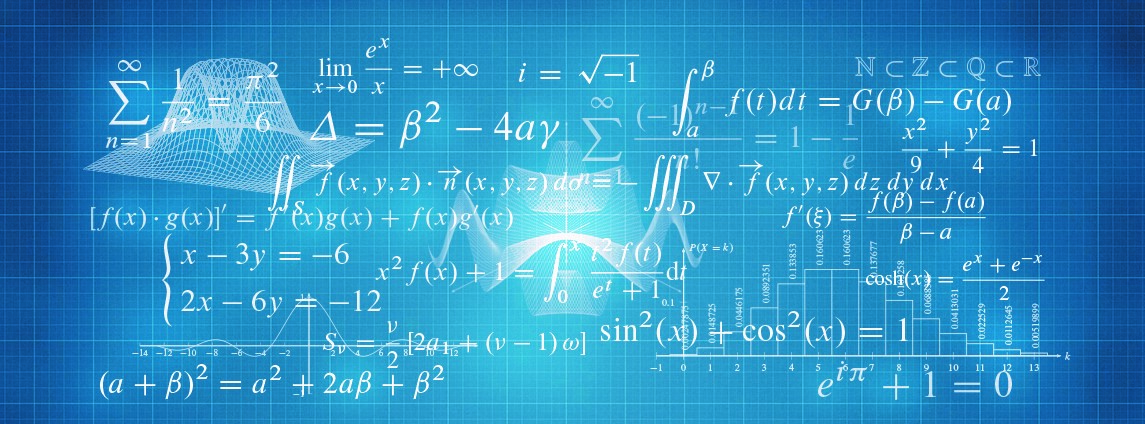
\includegraphics[width=17cm]{Kefalaio}};
\node[anchor=west,xshift=.08\paperwidth,yshift=.1\paperheight,rectangle]
{{\color{white}\fontsize{30}{20}\textbf{\textcolor{black}{\contour{white}{ΚΕΦΑΛΑΙΟ}}}}};
\node[anchor=west,xshift=.07\paperwidth,yshift=.05\paperheight,rectangle] {\fontsize{27}{20} {\color{black}{{\textcolor{black}{\contour{white}{\sc##1}}}}}};
%\fill[fill=black] (12.2,2) rectangle (14.8,4.7);
\node[anchor=west,xshift=.77\paperwidth,yshift=.077\paperheight,rectangle]
{\fontsize{80}{20}\textbf{\textit{\contour{black}{\thechapter}}}};
\end{tikzpicture}
};
\end{tikzpicture}
}
\titlespacing*{\chapter}{0pt}{20pt}{30pt}
}
%------------------------------------------------

\usepackage[outline]{contour}
\newcommand{\regularchapter}{%
\titleformat{\chapter}[display]
{\normalfont\huge\bfseries}{\chaptertitlename\ \thechapter}{20pt}{\Huge##1}
\titlespacing*{\chapter}
{0pt}{-20pt}{40pt}
}

\apptocmd{\mainmatter}{\fancychapter}{}{}
\apptocmd{\backmatter}{\regularchapter}{}{}
\apptocmd{\frontmatter}{\regularchapter}{}{}

\titlespacing*{\section}
{0pt}{30pt}{0pt}
\usepackage{booktabs}
\usepackage{hhline}
\DeclareRobustCommand{\perthousand}{%
\ifmmode
\text{\textperthousand}%
\else
\textperthousand
\fi}

\newcounter{typos}[chapter]
\renewcommand{\thetypos}{T\arabic{typos}}   
\newcommand{\Typos}{\refstepcounter{typos}\textcolor{gray}{\textbf{\thetypos}}}{}


\contentsmargin{0cm}
\titlecontents{part}[-1pc]
{\addvspace{10pt}%
\bf\Large ΜΕΡΟΣ\quad }%
{}
{}
{\;\dotfill\;\normalsize\ Σελίδα}%
%------------------------------------------
\titlecontents{chapter}[0pc]
{\addvspace{30pt}%
\begin{tikzpicture}[remember picture, overlay]%
\draw[fill=black,draw=black] (-.3,.5) rectangle (3.7,1.1); %
\pgftext[left,x=0cm,y=0.75cm]{\color{white}\sc\Large\bfseries Κεφάλαιο\ \thecontentslabel};%
\end{tikzpicture}\large\sc}%
{}
{}
{\hspace*{-2.3em}\hfill\normalsize Σελίδα \thecontentspage}%
\titlecontents{section}[2.4pc]
{\addvspace{1pt}}
{\contentslabel[\thecontentslabel]{2pc}}
{}
{\;\dotfill\;\small \thecontentspage}
[]
\titlecontents*{subsection}[4pc]
{\addvspace{-1pt}\small}
{}
{}
{\ --- \small\thecontentspage}
[ \textbullet\ ][]

\makeatletter
\renewcommand{\tableofcontents}{%
\chapter*{%
\vspace*{-20\p@}%
\begin{tikzpicture}[remember picture, overlay]%
\pgftext[right,x=12cm,y=0.2cm]{\Huge\sc\bfseries \contentsname};%
\draw[fill=black,draw=black] (9.5,-.75) rectangle (12.5,1);%
\clip (9.5,-.75) rectangle (15,1);
\pgftext[right,x=12cm,y=0.2cm]{\color{white}\Huge\bfseries \contentsname};%
\end{tikzpicture}}%
\@starttoc{toc}}
\makeatother
\pgfmathdeclarefunction{gauss}{2}{%
\pgfmathparse{1/(#2*sqrt(2*pi))*exp(-((x-#1)^2)/(2*#2^2))}%
}
\usepackage[contents={},scale=1,opacity=1,color=black,angle=0]{background}

\newcommand\blfootnote[1]{%
\begingroup
\renewcommand\thefootnote{}\footnote{#1}%
\addtocounter{footnote}{-1}%
\endgroup
}
\usepackage{epstopdf}
\epstopdfsetup{update}
\usepackage{textcomp}
\titleformat{\section}
{\normalfont\Large\bf}%
{}{0em}%
{{\color{black}\titlerule[1pt]}\vskip-.2\baselineskip{\parbox[t]{\dimexpr\textwidth-2\fboxsep\relax}{\raggedright\strut\thesection~#1\strut}}}[\vskip 0\baselineskip{\color{black}\titlerule[1pt]}]
\titlespacing*{\section}{0pt}{0pt}{0pt}

\newcommand{\methodologia}{\begin{center}
{\large \textbf{ΜΕΘΟΔΟΛΟΓΙΑ}}\\\vspace{-2mm}
\begin{tikzpicture}
\shade[left color=white, right color=black] (-3cm,0) rectangle (0,.2mm);
\shade[left color=black, right color=white] (0,0) rectangle (3cm,.2mm);   
\end{tikzpicture}
\end{center}}

\newcommand{\orismoi}{\begin{center}
\large \textcolor{\xrwma}{\textbf{ΟΡΙΣΜΟΙ}}\\\vspace{-2mm}
\begin{tikzpicture}
\shade[left color=white, right color=\xrwma] (-3cm,0) rectangle (0,.2mm);
\shade[left color=\xrwma, right color=white] (0,0) rectangle (3cm,.2mm);   
\end{tikzpicture}
\end{center}}
\newcommand{\thewrhmata}{\begin{center}
{\large \textcolor{\xrwmath}{\textbf{ΘΕΩΡΗΜΑΤΑ - ΠΟΡΙΣΜΑΤΑ - ΠΡΟΤΑΣΕΙΣ\\ΚΡΙΤΗΡΙΑ - ΙΔΙΟΤΗΤΕΣ}}}\\\vspace{-2mm}
\begin{tikzpicture}
\shade[left color=white, right color=\xrwmath,] (-5cm,0) rectangle (0,.2mm);
\shade[left color=\xrwmath, right color=white,] (0,0) rectangle (5cm,.2mm);   
\end{tikzpicture}
\end{center}}
\usepackage[labelfont={footnotesize,it,bf},font={footnotesize}]{caption}

\usepackage{wrapfig,wrap-rl}
%-------- ΜΑΘΗΜΑΤΙΚΑ ΕΡΓΑΛΕΙΑ ---------
\usepackage{mathtools}
%----------------------
%-------- ΠΙΝΑΚΕΣ ---------
\usepackage{booktabs}
%----------------------
%----- ΥΠΟΛΟΓΙΣΤΗΣ ----------
%\usepackage{calculator}
%----------------------------
\newcommand{\tss}[1]{\textsuperscript{#1}}
\newcommand{\tssL}[1]{\MakeLowercase{\textsuperscript{#1}}}
%----- ΟΡΙΖΟΝΤΙΑ ΛΙΣΤΑ ------
\usepackage{xparse}
\newcounter{answers}
\renewcommand\theanswers{\arabic{answers}}
\ExplSyntaxOn
\NewDocumentCommand{\results}{m}
{
\seq_set_split:Nnn \l_results_a_seq {,}{#1}
\par\nobreak\noindent\setcounter{answers}{0}
\seq_map_inline:Nn \l_results_a_seq
{
\makebox[.18\linewidth][l]{\stepcounter{answers}\theanswers.~##1}\hfill
}
\par
}
\seq_new:N \l_results_a_seq
\ExplSyntaxOff
%----------------------------

\usepackage{microtype}
\usepackage{float}
\usepackage{caption}
%----------- ΓΡΑΦΙΚΕΣ ΠΑΡΑΣΤΑΣΕΙΣ ---------
\pgfkeys{/pgfplots/aks_on/.style={axis lines=center,
xlabel style={at={(current axis.right of origin)},xshift=1.5ex, anchor=center},
ylabel style={at={(current axis.above origin)},yshift=1.5ex, anchor=center}}}
\pgfkeys{/pgfplots/grafikh parastash/.style={\xrwma,line width=.4mm,samples=200}}
\pgfkeys{/pgfplots/belh ar/.style={tick label style={font=\scriptsize},axis line style={-latex}}}
%-----------------------------------------

%---- ΟΡΙΖΟΝΤΙΟ - ΚΑΤΑΚΟΡΥΦΟ - ΠΛΑΓΙΟ ΑΓΚΙΣΤΡΟ ------
\newcommand{\orag}[3]{\node at (#1)
{$ \overcbrace{\rule{#2mm}{0mm}}^{{\scriptsize #3}} $};}

\newcommand{\kag}[3]{\node at (#1)
{$ \undercbrace{\rule{#2mm}{0mm}}_{{\scriptsize #3}} $};}

\newcommand{\Pag}[4]{\node[rotate=#1] at (#2)
{$ \overcbrace{\rule{#3mm}{0mm}}^{{\rotatebox{-#1}{\scriptsize$#4$}}}$};}
%-----------------------------------------
\tikzstyle{pl}=[line width=0.3mm]
\tikzstyle{plm}=[line width=0.4mm]
\tkzSetUpPoint[size=7,fill=white]
\newlist{rlist}{enumerate}{3}
\setlist[rlist]{itemsep=0mm,label=\roman*.}
\setlist[itemize]{itemsep=0mm}
\definecolor{bblue}{HTML}{4F81BD}
\definecolor{rred}{HTML}{C0504D}
\definecolor{ggreen}{HTML}{9BBB59}
\definecolor{ppurple}{HTML}{9F4C7C}

\makeatletter
\usetikzlibrary{patterns}
\tikzstyle{chart}=[
legend label/.style={font={\scriptsize},anchor=west,align=left},
legend box/.style={rectangle, draw, minimum size=5pt},
axis/.style={black,semithick,->},
axis label/.style={anchor=east,font={\tiny}},
]

\tikzstyle{bar chart}=[
chart,
bar width/.code={
\pgfmathparse{##1/2}
\global\let\bar@w\pgfmathresult
},
bar/.style={very thick, draw=white},
bar label/.style={font={\bf\small},anchor=north},
bar value/.style={font={\footnotesize}},
bar width=.75,
]

\tikzstyle{pie chart}=[
chart,
slice/.style={line cap=round, line join=round,thick,draw=white},
pie title/.style={font={\bf}},
slice type/.style 2 args={
##1/.style={fill=##2},
values of ##1/.style={}
}
]

\pgfdeclarelayer{background}
\pgfdeclarelayer{foreground}
\pgfsetlayers{background,main,foreground}


\newcommand{\pie}[3][]{
\begin{scope}[#1]
\pgfmathsetmacro{\curA}{90}
\pgfmathsetmacro{\r}{1}
\def\c{(0,0)}
\node[pie title] at (90:1.3) {#2};
\foreach \v/\s/\l in{#3}{
\pgfmathsetmacro{\deltaA}{\v/100*360}
\pgfmathsetmacro{\nextA}{\curA + \deltaA}
\pgfmathsetmacro{\midA}{(\curA+\nextA)/2}

\path[slice,\s] \c
-- +(\curA:\r)
arc (\curA:\nextA:\r)
-- cycle;
\pgfmathsetmacro{\d}{max((\deltaA * -(.5/50) + 1) , .5)}

\begin{pgfonlayer}{foreground}
\path \c -- node[pos=\d,pie values,values of \s]{$\l$} +(\midA:\r);
\end{pgfonlayer}

\global\let\curA\nextA
}
\end{scope}
}

\newcommand{\legend}[2][]{
\begin{scope}[#1]
\path
\foreach \n/\s in {#2}
{
++(0,-10pt) node[\s,legend box] {} +(5pt,0) node[legend label] {\n}
}
;
\end{scope}
}
\definecolor{a}{cmyk}{0,1,1,0.05}
\definecolor{b}{cmyk}{0,.8,.8,.15}
\definecolor{c}{cmyk}{0,.8,.8,.0}
\definecolor{d}{cmyk}{0,.7,.7,0}
\definecolor{e}{cmyk}{0,.5,.5,0}


\pgfplotsset{every axis/.append style={
x tick label style={/pgf/number format/.cd, 1000 sep={.}}}}
\newcommand{\shmeio}[2]{
\foreach \a in {1,...,#2}{
\node[dot] at (#1+.5,\a/2-.2){};}}

\newfontfamily\scfont{GFS Artemisia}
\font\icon = "Webdings"
\font\icons = "IcoMoon-Free"
\font\myfont = "Wingdings"
\font\mymath = "MyMathSymbols" at 16pt
\newcommand{\titlos}[3]{
\begin{center}
{\large {\textcolor{\xrwma}{\scfont\textsc{Σπύρος}}\,\,\textcolor{\xrwma}{\scfont\textsc{Φρόνιμος}}} - {\scfont\textsc{Μαθηματικός}}}
\\{\myfont\XeTeXglyph13} : spyrosfronimos@gmail.com\,\,|\,\,{\icons\XeTeXglyph188} : 6932327283 - 6974532090\\
\rule{12.7cm}{.1mm}\\
\vspace{2mm}
ΣΗΜΕΙΩΣΕΙΣ ΘΕΩΡΙΑΣ - ΟΡΙΣΜΟΙ ΚΑΙ ΘΕΩΡΗΜΑΤΑ\\
\vspace{1mm}
{\bf\today}
\end{center}
\vspace{.5cm}
\begin{center}
{\Large\bf\MakeUppercase{#1}}
\end{center}
\begin{center}
\textbf{{\Huge \textcolor{\xrwma}{#2}}}
\end{center}
\vspace{-5mm}
\begin{center}
{\Large\bf{\MakeUppercase{#3}}}
\end{center}
\vspace{1cm}}



\begin{document}
\pagenumbering{gobble}% Remove page numbers (and reset to 1)
\clearpage
\backmatter
\pagestyle{empty}
\titlos{B΄ ΓΥΜΝΑΣΙΟΥ}{Μαθηματικά}{Ορισμοί και θεωρήματα}
\vspace{1cm}
\begin{center}
\begin{tikzpicture}[scale=1.2]
\tkzDefPoint(0,0){B}
\tkzDefPoint(3.5,0){C}
\tkzDefPoint(0,2.1){A}
\tkzMarkRightAngle[size=.2](C,B,A)
\draw[pl](A)--(B)--(C)--cycle;
\tkzDrawPoints(A,B,C)
\tkzLabelPoint[above left](A){$B$}
\tkzLabelPoint[left](B){$A$}
\tkzLabelPoint[right](C){$\varGamma$}
\node at (1.75,-0.25) {\footnotesize$\beta$};
\node at (-0.25,1) {\footnotesize$\gamma$};
\node at (2,1.25) {\footnotesize$a$};
\node at (2,2.5) {$B\varGamma^2=AB^2+A\varGamma^2$};
\end{tikzpicture}\mbox{}\\
\vspace{3cm}
\begin{minipage}{7cm}
\begin{center}
ΑΝΑΛΥΤΙΚΟ ΤΥΠΟΛΟΓΙΟ ΓΙΑ ΤΗ ΘΕΩΡΙΑ ΤΩΝ ΜΑΘΗΜΑΤΙΚΩΝ Β΄ ΓΥΜΝΑΣΙΟΥ
\end{center}
\end{minipage}
\end{center}
\vspace*{\fill{\begin{center}
\end{center}}}
\pagenumbering{arabic}
\mainmatter
\pagestyle{fancy}
\chapter{Εξισώσεις - Ανισώσεις}
\section{Αλγεβρικές Παραστάσεις}\mbox{}\\
\orismoi
\Orismos{Μεταβλητή}
Μεταβλητή ονομάζεται το γράμμα ή το σύμβολο που χρησιμοποιούμε για να συμβολίσουμε έναν άγνωστο αριθμό. Χρησιμοποιούμε οποιοδήποτε γράμμα του ελληνικού ή του λατινικού αλφαβήτου όπως $ a,\beta,x,y,\ldots $\\\\
\Orismos{ΑΡΙΘΜΗΤΙΚΗ ΠΑΡΑΣΤΑΣΗ}
Αριθμητική ονομάζεται κάθε παράσταση η οποία περιέχει πράξεις μεταξύ αριθμών.\\\\
\Orismos{ΑΛΓΕΒΡΙΚΗ ΠΑΡΑΣΤΑΣΗ}
Αλγεβρική ονομάζεται κάθε παράσταση η οποία περιέχει πράξεις μεταξύ αριθμών και μεταβλητών.
\begin{itemize}[itemsep=0mm]
\item \textbf{Tιμή} μιας αλγεβρικής παράστασης ονομάζεται το αποτέλεσμα που προκύπτει ύστερα από πράξεις εαν αντικατασταθούν οι μεταβλητές της με αριθμούς.
\item Κάθε προσθετέος μέσα σε μια αλγεβρική παράσταση ονομάζεται \textbf{όρος} της παράστασης.
\end{itemize}
\Orismos{ΑΝΑΓΩΓΉ ΟΜΟΊΩΝ ΌΡΩΝ}
Αναγωγή ομοίων όρων ονομάζεται η διαδικασία με την οποία απλοποιούμε μια αλγεβρική παράσταση προσθέτοντας τoυς όμοιους όρους της.\\\\
\thewrhmata
\Thewrhma{Επιμεριστική Ιδιότητα}
Αν $ a,\beta,\gamma $ είναι τρεις οποιοιδήποτε αριθμοί τότε το γινόμενο του ενός με το άθροισμα των άλλων δίνεται από τον παρακάτω τύπο :
\[ a\cdot(\beta+\gamma)=a\cdot\beta+a\cdot\gamma \]
\section{Εξισώσεις}\mbox{}\\
\orismoi
\Orismos{Εξίσωση}
Εξίσωση ονομάζεται κάθε ισότητα που περιέχει τουλάχιστον μια μεταβλητή. Μια εξίσωση με έναν άγνωστο θα έιναι της μορφής :
\[ ax+\beta=0 \]
όπου $ a,\beta $ είναι οποιοιδήποτε αριθμοί.
\begin{itemize}[itemsep=0mm]
\item Μια εξίσωση αποτελείται από \textbf{2 μέλη}, τα οποία είναι τα μέρη της δεξιά και αριστερά του $ = $.
\[ \textrm{1\tss{ο} μέλος}=\textrm{2\tss{ο} μέλος} \]
\item \textbf{Άγνωστοι} ονομάζονται οι όροι της εξίσωσης οι οποίοι περιέχουν τη μεταβλητή, ενώ \textbf{γνωστοί} ονομάζονται οι αριθμοί δηλαδή οι σταθεροί όροι της εξίσωσης.
\item Κάθε αριθμός που επαληθεύει μια εξίσωση ονομάζεται \textbf{λύση} της εξίσωσης.
\item Η διαδικασία με την οποία βρίσκουμε τη λύση μιας εξίσωσης ονομάζεται \textbf{επίλυση}.
\item Εαν μια εξίσωση έχει λύσεις όλους τους πραγματικούς αριθμούς ονομάζεται \textbf{ταυτότητα} ή \textbf{αόριστη}.
\item Εαν μια εξίσωση δεν έχει καμία λύση ονομάζεται \textbf{αδύνατη}.
\end{itemize}
\Orismos{επαληθευση}
Επαλήθευση ονομάζεται η διαδικασία με την οποία εξετάζουμε αν ένας αριθμός είναι λύση μιας εξίσωσης, αντικαθιστώντας τη μεταβλητή της εξίσωσης με τον αριθμό αυτό.\\\\
\thewrhmata
\Thewrhma{Ιδιότητεσ ισοτήτων}
Σε κάθε ισότητα εαν τοποθετήσουμε τον ίδιο αριθμό και στα δύο μέλη της με πρόσθεση, αφαίρεση, πολλαπλασιασμό ή διαίρεση, η σχέση που προκύπτει είναι ξανά ισότητα :
\[ a=\beta\Rightarrow
\begin{cases}
a+\gamma=\beta+\gamma\\a-\gamma=\beta-\gamma
\end{cases}\ \ \textrm{ και }\ \ \begin{aligned}
&a\cdot\gamma=\beta\cdot\gamma\\&\dfrac{a}{\gamma}=\dfrac{\beta}{\gamma}\;\;,\;\;\gamma\neq0
\end{aligned} \]
\Thewrhma{Πράξεισ κατά μέλη}
Προσθέτοντας κατά μέλη κάθε ζεύγος ισοτήτων $ a=\beta $ και $ \gamma=\delta $ προκύπτει ισότητα, με 1\textsuperscript{ο} μέλος το άθροισμα των 1\textsuperscript{ων} μελών τους και 2\textsuperscript{ο} μέλος το άθροισμα των 2\textsuperscript{ων} μελών τους. Η ιδιότητα αυτή ισχύει και για αφαίρεση, πολλαπλασιασμό και διάιρεση κατά μέλη.
\[ \textrm{Αν }a=\beta\;\;\textrm{και}\;\;\gamma=\delta\Rightarrow\ccases{\textrm{\textbf{\textit{1. Πρόσθεση κατά μέλη }}}& a+\gamma=\beta+\delta\\\textrm{\textbf{\textit{2. Αφαίρεση κατά μέλη }}}& a-\gamma=\beta-\delta\\\textrm{\textbf{\textit{3. Πολλαπλασιασμός κατά μέλη }}}& a\cdot\gamma=\beta\cdot\delta\\\textrm{\textbf{\textit{4. \boldmath$ \varDelta $ιαίρεση κατά μέλη }}}& \dfrac{a}{\gamma}=\dfrac{\beta}{\delta}\;\;,\;\;\gamma\cdot\delta\neq0} \]
\section{Ανισώσεις}\mbox{}\\
\orismoi
\Orismos{Ανίσωση}
Ανίσωση ονομάζεται κάθε ανισότητα η οποία περιέχει τουλάχιστον μια μεταβλητή. Μια ανίσωση μιας μεταβλητής θα έχει τη μορφή
\[ ax+\beta>0\textrm{ ή }ax+\beta<0 \]
όπου $ a,\beta $ οποιοιδήποτε αριθμοί.
\begin{itemize}[itemsep=0mm]
\item Ανισώσεις αποτελούν και οι σχέσεις με σύμβολα ανισοϊσότητας $ \leq,\geq $.
\item Κάθε αριθμός που επαληθεύει μια ανίσωση ονομάζεται \textbf{λύση} της. Κάθε ανίσωση έχει λύσεις ένα \textbf{σύνολο αριθμών}.
\item Αν μια ανίσωση έχει λύσεις όλους τους αριθμούς ονομάζεται \textbf{αόριστη}.
\item Αν μια ανίσωση δεν έχει καθόλου λύσεις ονομάζεται \textbf{αδύνατη}.
\item Σχέσεις τις μορφής $ Q(x)\leq P(x)\leq R(x) $ λέγονται \textbf{διπλές ανισώσεις} όπου $ P(x),Q(x),R(x) $ είναι αλγεβρικές παρατάσεις. Αποτελείται από δύο ανισώσεις, με κοινό μέλος την παράσταση $ P(x) $, οι οποίες συναληθεύουν.
\item \textbf{Κοινές λύσεις} μιας διπλής ανίσωσης ή δύο ή περισσότερων ανισώσεων ονομάζονται οι αριθμοί που επαληθεύουν όλες τις ανισώσεις συγχρόνως.
\end{itemize}

\thewrhmata
\Thewrhma{ΙΔΙΟΤΗΤΕΣ ΑΝΙΣΟΤΗΤΩΝ}\label{th:idan}
\vspace{-5mm}
\begin{enumerate}
\item Εαν σε μια ανισότητα προσθέσουμε ή αφαιρέσουμε τον ίδιο αριθμό και απ' τα δύο μέλη της, προκύπτει ξανά ανισότητα με την ίδια φορά της αρχικής.
\[ a>\beta\Leftrightarrow\ccases{a+\gamma>\beta+\gamma\\a-\gamma>\beta-\gamma} \]
\item Για να πολλαπλασιάσουμε ή να διαιρέσουμε και τα δύο μέλη μιας ανισότητας με τον ίδιο αριθμό διακρίνουμε τις εξής περπτώσεις :
\begin{rlist}
\item Εαν πολλαπλασιάσουμε ή διαιρέσουμε και τα δύο μέλη μιας ανισότητας με τον ίδιο \textbf{θετικό} αριθμό, τότε προκύπτει ανισότητα με την \textbf{ίδια} φορά της αρχικής.
\item Εαν πολλαπλασιάσουμε ή διαιρέσουμε και τα δύο μέλη μιας ανισότητας με τον ίδιο \textbf{αρνητικό} αριθμό, τότε προκύπτει ανισότητα με φορά \textbf{αντίθετη} της αρχικής.
\end{rlist}
\begin{gather*}
\textrm{Αν }\gamma>0\textrm{ τότε }a>\beta\Leftrightarrow a\cdot\gamma>\beta\cdot\gamma\textrm{ και }\dfrac{a}{\gamma}>\dfrac{\beta}{\gamma}\\
\textrm{Αν }\gamma<0\textrm{ τότε }a>\beta\Leftrightarrow a\cdot\gamma<\beta\cdot\gamma\textrm{ και }\dfrac{a}{\gamma}<\dfrac{\beta}{\gamma}
\end{gather*}
\end{enumerate}
Ανάλογα συμπεράσματα ισχύουν και για τις ανισότητες $ a<\beta,a\geq\beta $ και $ a\leq\beta $.\\\\
\Thewrhma{Πράξεισ κατά μέλη ανισοτήτων}
Προσθέτοντας κατά μέλη κάθε ζεύγος ανισοτήτων προκύπτει ανισότητα, με 1\textsuperscript{ο} μέλος το άθροισμα των 1\textsuperscript{ων} μελών τους και 2\textsuperscript{ο} μέλος το άθροισμα των 2\textsuperscript{ων} μελών τους με φορά ίδια της αρχικής. Ομοίως πολλαπλασιάζοντας κατά μέλη δύο ανισότητες προκύπτει ανισότητα με φορά ίδια της αρχικής. Για να πολλαπλασιαστούν δύο ανισότητες κατά μέλη πρέπει όλοι οι όροι τους να είναι θετικοί.
\[ a>\beta\;\;\textrm{και}\;\;\gamma>\delta\Rightarrow\ccases{\textrm{\textbf{\textit{1. Πρόσθεση κατά μέλη }}}& a+\gamma>\beta+\delta\\\textrm{\textbf{\textit{2. Πολλαπλασιασμός κατά μέλη }}}& a\cdot\gamma>\beta\cdot\delta\;\;,\;\;\textrm{με }a,\beta,\gamma,\delta>0} \]
\textbf{Δεν} μπορούμε να αφαιρέσουμε ή να διαιρέσουμε ανισότητες κατά μέλη.\\\\
\chapter{Πραγματικοί Αριθμοί}
\section{Τετραγωνική ρίζα}\mbox{}\\
\orismoi
\Orismos{Τετραγωνική Ρίζα}
Τετραγωνική ρίζα ενός θετικού αριθμού $ x $ ονομάζεται ο \textbf{θετικός} αριθμός $ a $ που αν υψωθεί στο τετράγωνο δίνει τον αριθμό $ x $  και συμβολίζεται με $ \sqrt{x} $.
\[ \sqrt{x}=a\;\;,\;\;\textrm{ όπου }x\geq0\textrm{ και }a\geq0 \]
\begin{itemize}[itemsep=0mm]
\item Ο αριθμός $ x $ ονομάζεται \textbf{υπόριζο}.
\item Δεν ορίζεται ρίζα αρνητικού αριθμού.
\end{itemize}

\thewrhmata
\Thewrhma{Ιδιότητεσ Ριζών}
Για οποιουσδήποτε αριθμούς $ x,y $ ισχύουν οι παρακάτω ιδιότητες που αφορούν την τετραγωνική τους ρίζα.
\begin{center}
\begin{tabular}{cc}
\hline \rule[-2ex]{0pt}{5.5ex} \textbf{Ιδιότητα} & \textbf{Συνθήκη} \\
\hhline{==}\rule[-2ex]{0pt}{5.5ex}  Τετράγωνο ρίζας & $ \left(\sqrt{x}\;\right)^2=x\;\;,\;\; x\geq0  $ \\
\rule[-2ex]{0pt}{5.5ex}  Ρίζα τετραγώνου & $ \sqrt{x^2}=|x|\;\;,\;\;x\textrm{ πραγματικός}$\\
\rule[-2ex]{0pt}{5.5ex}  Ρίζα γινομένου & $ \sqrt{x\cdot y}=\!\sqrt{x}\cdot\!\sqrt{y}\;\;,\;\; x,y\geq0 $ \\
\rule[-2ex]{0pt}{6.5ex} Ρίζα πηλίκου & $ \sqrt{\dfrac{x}{y}}\;=\dfrac{\sqrt{x}}{\sqrt{y}}\;\;,\;\;x\geq0\textrm{ και }y>0 $\vspace{1mm} \\
\hline
\end{tabular}
\end{center}
\section{Άρρητοι - Πραγματικοί αριθμοί}\mbox{}\\
\orismoi
\Orismos{Ρητός - άρρητος αριθμός}
Ρητός ονομάζεται ο αριθμός ο οποίος μπορεί να γραφτεί στη μορφή κλάσματος $ \frac{a}{\beta} $ με ακέραιους όρους $ a,\beta $. Κάθε αριθμός που δεν είναι ρητός ονομάζεται \textbf{άρρητος}.\\\\\\
\Orismos{Άξονασ των πραγματικών αριθμών}
Ο άξονας των πραγματικών αριθμών είναι μια αριθμημένη ευθεία στην οποία μπορούν να τοποθετηθούν όλοι οι πραγματικοί αριθμοί σε αύξουσα σειρά από τα αριστερά προς τα δεξιά. \textbf{Αρχή} του άξονα είναι το σημείο $ O $ στο οποίο βρίσκεται ο αριθμός $ 0 $.
\begin{center}
\begin{tikzpicture}
\tkzInit[xmin=-4,xmax=4]
\draw[-latex] (-5,0) -- coordinate (x axis mid) (5.4,0) node[right,fill=white] {{\footnotesize $ x $}};
\foreach \x in {-5,-4,-3,...,5}
\draw (\x,.5mm) -- (\x,-.5mm) node[anchor=north,fill=white] {{\scriptsize \x}};
\draw[latex-|] (-5,0.7) --  (-0.02,0.7);
\draw[|-latex] (0.02,0.7) --  (5,0.7);
\tkzText(-2,0.85){Αρνητικοί Αριθμοί}
\tkzText(2,0.85){Θετικοί Αριθμοί}
\tkzDefPoint(3,0){A}
\tkzDefPoint(1.4142,0){B}
\tkzDefPoint(-1.5,0){C}
\tkzDefPoint(-2.7,0){D}
\tkzDrawPoints[size=7,fill=white](A,B,C,D)
\tkzLabelPoint[above](A){{\scriptsize $ A(3) $}}
\tkzLabelPoint[above](B){{\scriptsize $ B\left(\!\! \sqrt{2}\right)  $}}
\tkzLabelPoint[above](C){{\scriptsize $ \varGamma\left(-\frac{3}{2} \right)  $}}
\tkzLabelPoint[above](D){{\scriptsize $ \varDelta(-2{,}7) $}}
\end{tikzpicture}
\end{center}
\begin{itemize}[itemsep=0mm]
\item Η θέση ενός αριθμού πάνω στην ευθεία σχεδιάζεται με ένα σημείο.
\item Ο αριθμός που βρίσκεται στη θέση αυτή ονομάζεται \textbf{τετμημένη} του σημείου.
\end{itemize}
\chapter{Συναρτήσεις}
\section{Η έννοια της συνάρτησης}\mbox{}\\
\orismoi
\Orismos{Συνάρτηση}
Συνάρτηση ονομάζεται μια σχέση που συνδέει δύο μεταβλητές $ x,y $ με την οποία \textbf{κάθε} τιμή της μεταβλητής $ x $ αντιστοιχεί σε \textbf{μια μόνο} τιμή της μεταβλητής $ y $.
\begin{itemize}[itemsep=0mm]
\item Κάθε συνάρτηση γράφεται σαν ισότητα η οποία περιέχει και τις δύο μεταβλητές. Η ισότητα αυτή λέγεται \textbf{εξίσωση} της συνάρτησης.
\item Αν $ y=A(x) $ όπου $ A(x) $ είναι μια αλγεβρική παράσταση του $ x $, τότε λέμε ότι η μεταβλητή $ y $ γραφεται \textbf{ως συνάρτηση} του $ x $.
\end{itemize}
\section{Γραφική παράσταση συνάρτησης}\mbox{}\\
\orismoi
\Orismos{Ορθογώνιο - Ορθοκανονικό Σύστημα Συντεταγμένων}
Ορθογώνιο σύστημα συντεταγμένων ονομάζεται το σχήμα που αποτελείται από δύο κάθετα τοποθετημένους μεταξύ τους άξονες αρίθμησης πάνω στους οποίους παίρνουν τιμές δύο μεταβλητές.
\begin{itemize}[itemsep=0mm]
\item Το σημείο τομής των δύο αξόνων ονομάζεται \textbf{αρχή των αξόνων}.
\item Σε κάθε άξονα του συστήματος, επιλέγουμε αυθαίρετα ένα μήκος το οποίο ορίζουμε ως μονάδα μέτρησης.
\item Εαν σε κάθε άξονα θέσουμε την ίδια μονάδα μέτρησης το σύστημα ονομάζεται \textbf{ορθοκανονικό}.
\item Ο οριζόντιος άξονας ονομάζεται \textbf{άξονας τετμημένων} και συμβολίζεται με $ x'x $.
\end{itemize}
\begin{minipage}{\linewidth}\mbox{}\\
\vspace{-1.2cm}
\begin{WrapText1}{10}{4.9cm}
\begin{tikzpicture}[scale=.48,y=1cm]
\tkzInit[xmin=-4,xmax=4.4,ymin=-4,ymax=4.4,ystep=1]
\draw[-latex]  (-4,0) node[left,fill=white] {{\footnotesize $ x' $}} -- coordinate (x axis mid) (4.4,0) node[right,fill=white] {{\footnotesize $ x $}};
\draw[-latex] (0,-4) node[below,fill=white] {{\footnotesize $ y' $}} -- (0,4.4) node[above,fill=white] {{\footnotesize $ y $}};
\draw (1,.15) -- (1,-.15) node[anchor=north] {\scriptsize 1};
\draw (.15,1) -- (-.15,1) node[anchor=east] {\scriptsize 1};
\tkzDefPoint(0,0){O}
\tkzDefPoint(2,1.8){M}
\tkzLabelPoint[below left](O){$ O $}
\tkzLabelPoint[right](M){{\footnotesize $ Μ(x,y) $}}
\draw[dashed] (0,1.8) node[left]{{\scriptsize $ y $}}--(2,1.8)--(2,0) node[below]{{\scriptsize $ x $}};
\tkzDrawPoint[size=7,fill=white](M)
\tkzText(2.2,3.3){{\scriptsize 1\textsuperscript{ο} Τεταρτημόριο}}
\tkzText(-2.2,3.3){{\scriptsize 2\textsuperscript{ο} Τεταρτημόριο}}
\tkzText(-2.2,-2){{\scriptsize 3\textsuperscript{ο} Τεταρτημόριο}}
\tkzText(2.2,-2){{\scriptsize 4\textsuperscript{ο} Τεταρτημόριο}}
\tkzText(2.2,2.7){{\scriptsize $ (+,+) $}}
\tkzText(-2.2,2.7){{\scriptsize $ (-,+) $}}
\tkzText(-2.2,-1.4){{\scriptsize $ (-,-) $}}
\tkzText(2.2,-1.4){{\scriptsize $ (+,-) $}}
\end{tikzpicture}
\end{WrapText1}
\begin{itemize}[itemsep=0mm]
\item Ο κατακόρυφος άξονας ονομάζεται \textbf{άξονας τεταγμένων} και συμβολίζεται με $ y'y $.
\item Κάθε σημείο του επιπέδου του συστήματος συντεταγμένων αντιστοιχεί σε ένα ζευγάρι αριθμών της μορφής $(x,y)$. Aντίστροφα, κάθε ζευγάρι αριθμών $(x,y)$ αντιστοιχεί σε ένα σημείο του επιπέδου.
\item Το ζεύγος αριθμών $(x,y)$ ονομάζεται \textbf{διατεταγμένο ζεύγος αριθμών} διότι έχει σημασία η διάταξη δηλαδή η σειρά με την οποία εμφανίζονται οι αριθμοί.
\item Οι αριθμοί $x,y$ ονομάζονται \textbf{συντεταγμένες} του σημείου στο οποίο αντιστοιχούν. Ο αριθμός $x$ ονομάζεται \textbf{τετμημένη} του σημείου ενώ ο $y$ \textbf{τεταγμένη}.
\end{itemize}\end{minipage}\mbox{}\\
\vspace{-2mm}
\begin{itemize}
\item Στον οριζόντιο άξονα $ x'x $, δεξιά της αρχής των αξόνων, βρίσκονται οι θετικές τιμές της μεταβλητής $x$ ενώ αριστερά, οι αρνητικές.
\item Αντίστοιχα στον κατακόρυφο άξονα $ y'y $, πάνω από την αρχή των αξόνων βρίσκονται οι θετικές τιμές της μεταβλητής $y$, ενώ κάτω οι αρνητικές τιμές.
\item Οι άξονες χωρίζουν το επίπεδο σε τέσσερα μέρη τα οποία ονομάζονται \textbf{τεταρτημόρια}. Ως 1\textsuperscript{ο} τεταρτημόριο ορίζουμε το μέρος στο οποίο ανήκουν οι θετικοί ημιάξονες $ Ox $ και $ Oy $.
\end{itemize}
\Orismos{Γραφική Παράσταση συνάρτησησ}
Γραφική παράσταση μιας συνάρτησης ονομάζεται το σύνολο των σημείων του επιπέδου $ M(x,y) $ των οποίων οι συντεταγμένες επαληθεύουν την εξίσωση της.\\
\begin{minipage}{\linewidth}\mbox{}\\
\vspace{-1.2cm}
\begin{WrapText1}{8}{4.4cm}
\vspace{-4mm}
\begin{tikzpicture}[scale=.7,domain=.2:4.5,y=.7cm]
\tkzInit[xmin=-.5,xmax=7,ymin=-.5,ymax=1.2,ystep=1]
\draw[-latex] (-.5,0) -- coordinate (x axis mid) (5,0) node[right,fill=white] {{\footnotesize $ x $}};
\draw[-latex] (0,-.5) -- (0,4.4) node[above,fill=white] {{\footnotesize $ y $}};
\draw[,domain=.3:3.7,samples=200,line width=.4mm,\xrwma] plot function{(x-2)**3-2*x+6};
\tkzDefPoint(1.5,2.875){A}
\tkzDrawPoint[size=7,fill=\xrwma,color=\xrwma](A)
\draw[dashed] (0,2.875) node[anchor=east]{{\scriptsize $ y $}}  -- (A) -- (1.5,0) node[anchor=north] {{\scriptsize $ x $}};
\tkzLabelPoint[above=1mm](A){{\footnotesize $ M\left( x,y\right)  $}}
\tkzDefPoint(0,0){O}
\tkzLabelPoint[below left](O){$ O $}
\end{tikzpicture}
\end{WrapText1}
\begin{itemize}[itemsep=0mm]
\item Το σύνολο των σημείων της παριστάνει σχήμα.
\item Η εξίσωση $ y=A(x) $ είναι η εξίσωση της γραφικής παραστασης την οποία επαληθεύουν οι συντεταγμένες των σημείων της.
\end{itemize}\end{minipage}\mbox{}\\\\\\
\section{Η συνάρτηση {$ \mathbold{y=ax} $}}\mbox{}\\
\orismoi
\Orismos{Η συνάρτηση \MakeLowercase{$ \mathbold{y=ax} $}}
\wrapr{-5mm}{7}{3.8cm}{-9mm}{\begin{tikzpicture}
\begin{axis}[x=1cm,y=.7cm,aks_on,xmin=-.5,xmax=3,
ymin=-.5,ymax=3,ticks=none,xlabel={\footnotesize $ x $},
ylabel={\footnotesize $ y $},belh ar]
\addplot[grafikh parastash,domain=-.5:2.7]{x};
\end{axis}
\node[fill=white,inner sep=.2mm] at (0.25,0.1) {$O$};
\node at (1.5,2) {{\footnotesize $y=ax$}};
\end{tikzpicture}}{
Η συνάρτηση $ y=ax $ είναι η συνάρτηση που συνδέει δύο \textbf{ανάλογα} ποσά $ x,y $.
\begin{itemize}[itemsep=0mm]
\item Η γραφική της παράσταση είναι ευθεία γραμμή η οποία διέρχεται από την αρχή των αξόνων.
\item Ο πραγματικός αριθμός $ a $ ονομάζεται \textbf{κλίση} της ευθείας. Ισούται με $ a=\frac{y}{x} $.
\end{itemize}}
\section{Η συνάρτηση {$ \mathbold{y=ax+\beta} $}}\mbox{}\\
\orismoi
\Orismos{Η συνάρτηση \MakeLowercase{$ \mathbold{y=ax+\beta} $}}
\wrapr{-5mm}{7}{3.8cm}{-9mm}{\begin{tikzpicture}
\begin{axis}[x=1cm,y=.7cm,aks_on,xmin=-.5,xmax=3,
ymin=-.5,ymax=3,ticks=none,xlabel={\footnotesize $ x $},
ylabel={\footnotesize $ y $},belh ar]
\addplot[grafikh parastash,domain=-.5:2.7,dashed]{x};
\addplot[grafikh parastash,domain=-.5:2]{x+1};
\end{axis}
\node[fill=white,inner sep=.2mm] at (0.25,0.1) {$O$};
\node at (1.5,2.5) {{\footnotesize $y=ax+\beta$}};
\draw[-latex] (1.5,1.05) -- (1.5,1.75);
\node at (1.35,1.35) {\footnotesize$\beta$};
\end{tikzpicture}}{
Η συνάρτηση $ y=ax+\beta $ παριστάνει ευθεία γραμμή η οποία είναι παράλληλη με την ευθεία $ y=ax $. \begin{itemize}[itemsep=0mm]
\item Ο αριθμός $ a $ ονομάζεται \textbf{κλίση} της ευθείας.
\item Η ευθεία $ y=ax+\beta $ με $ \beta\neq0 $ αποτελεί κατακόρυφη μετατόπιση της ευθείας $ y=ax $ ίση με $ \beta $ μονάδες.
\end{itemize}}
\thewrhmata
\Thewrhma{Η συνάρτηση \MakeLowercase{$ \mathbold{ax+\beta y=\gamma} $}}
Η εξίσωση $ ax+\beta y=\gamma $ παριστάνει ευθεία γραμμή αν ισχύει $ a\neq0 $ ή $ \beta\neq0 $.
\begin{itemize}[itemsep=0mm]
\item Οι εξισώσεις της μορφής $ y=\kappa $ παριστάνουν οριζόντιες ευθείες.
\item Οι εξισώσεις της μορφής $ x=\kappa $ παριστάνουν κατακόρυφες ευθείες.
\end{itemize}
\section{Η συνάρτηση {$ \mathbold{y=\frac{a}{x}} $}}\mbox{}\\
\orismoi
\Orismos{Η συνάρτηση \MakeLowercase{$ \mathbold{y=\frac{a}{x}} $}}
\wrapr{-5mm}{7}{4.5cm}{-10mm}{\begin{tikzpicture}
\begin{axis}[x=.7cm,y=.7cm,aks_on,xmin=-3,xmax=3,
ymin=-2.8,ymax=3,ticks=none,xlabel={\footnotesize $ x $},
ylabel={\footnotesize $ y $},belh ar]
\addplot[grafikh parastash,domain=.19:2.7]{.5/x};
\addplot[grafikh parastash,domain=-2.7:-.19]{.5/x};
\end{axis}
\node[fill=white,inner sep=.2mm] at (1.85,1.75) {$O$};
\node at (1.25,3) {$y=\frac{a}{x}$};
\end{tikzpicture}}{
Η συνάρτηση $ y=\frac{a}{x} $ είναι η συνάρτηση η οποία συνδέει δύο αντιστρόφως ανάλογα ποσά $ x,y $.
\begin{itemize}[itemsep=0mm]
\item Η γραφική της παράσταση ονομάζεται \textbf{υπερβολή}. Αποτελείται από δύο κλάδους όπως φαίνεται στο σχήμα.
\item Ο αριθμός $ a $ είναι διάφορος του μηδενός.
\end{itemize}}
\thewrhmata
\Thewrhma{Η συνάρτηση \MakeLowercase{$ \mathbold{y=\frac{a}{x}} $}}
Για τη γραφική παράσταση της συνάρτησης $ y=\frac{a}{x} $ ισχύουν τα εξής:
\begin{rlist}
\item Η υπερβολή έχει κέντρο συμμετρίας την αρχή των αξόνων.
\item Οι άξονες $ x'x $ και $ y'y $ είναι άξονες συμμετρίας της υπερβολής.
\item Αν $ a>0 $ η υπερβολή βρίσκεται στο 1\tss{ο} και στο 3\tss{ο} τεταρτημόριο ενώ αν $ a<0 $ βρίσκεται στο 2\tss{ο} και στο 4\tss{ο} τεταρτημόριο.
\end{rlist}
\begin{center}
\begin{tikzpicture}
\begin{axis}[x=.7cm,y=.7cm,aks_on,xmin=-3,xmax=3,
ymin=-2.8,ymax=3,ticks=none,xlabel={\footnotesize $ x $},
ylabel={\footnotesize $ y $},belh ar]
\addplot[grafikh parastash,domain=.19:2.7]{.5/x};
\addplot[grafikh parastash,domain=-2.7:-.19]{.5/x};
\end{axis}
\node[fill=white,inner sep=.2mm] at (1.85,1.75) {$O$};
\node at (1.25,3) {$y=\frac{a}{x}$};
\node at (1.25,2.5) {$a>0$};
\end{tikzpicture}\qquad\begin{tikzpicture}
\begin{axis}[x=.7cm,y=.7cm,aks_on,xmin=-3,xmax=3,
ymin=-2.8,ymax=3,ticks=none,xlabel={\footnotesize $ x $},
ylabel={\footnotesize $ y $},belh ar]
\addplot[grafikh parastash,domain=.19:2.7]{-.5/x};
\addplot[grafikh parastash,domain=-2.7:-.19]{-.5/x};
\end{axis}
\node[fill=white,inner sep=.2mm] at (1.85,1.75) {$O$};
\node at (3,3) {$y=\frac{a}{x}$};
\node at (3,2.5) {$a<0$};
\end{tikzpicture}
\end{center}
\chapter{Εμβαδά - Πυθαγόριεο Θεώρημα}
\section{Εμβαδόν επίπεδης επιφάνειας}\mbox{}\\
\orismoi
\Orismos{Εμβαδόν}
Εμβαδόν μιας επίπεδης επιφάνειας ονομάζεται ο θετικός αριθμός ο οποίος εκφράζει το μέγεθος της έκτασης που καταλαμβάνει η επιφάνεια αυτή.\\\\
\Orismos{Μονάδα μέτρησης}
Μονάδα μέτρησης επιφάνειας ονομάζεται μια επιφάνεια οποιουδήποτε σχήματος η οποία χρησιμοποιείται για η μέτρηση και σύγκριση όλων των επιφανειών.\\\\
\section{Μονάδες μέτρησης επιφάνειας}\mbox{}\\
\orismoi
\Orismos{Βασικές μονάδες μέτρησης επιφάνειας}
Στον παρακάτω πίνακα βλέπουμε τις βασικές μονάδες μέτρησης επιφανειών που χρησιμοποιούμε καθώς και τις σχέσεις που τις συνδέουν στο διάγραμμα που ακολουθεί:
\begin{center}
\textbf{ ΕΠΙΦΑΝΕΙΑ}\\\vspace{2mm}
\begin{tabular}{ccc}
\hline \rule[-2ex]{0pt}{5.5ex}\textbf{Μονάδα Μέτρησης} & \textbf{Συμβολισμός} & \textbf{Σχέσεις μεταξύ Μ.Μ.} \\ 
\hhline{===} \rule[-2ex]{0pt}{5.5ex} \textbf{Τ.Χιλιόμετρο} & $ 1km^2 $ & $ 1km^2=1000\textrm{ στρέμματα}=10^6m^2 $ \\ 
\rule[-2ex]{0pt}{4ex} \textbf{Στρέμμα} & $ 1\textrm{ στρέμμα} $ & $ \frac{1}{1000}km^2=1\textrm{ στρέμμα}=1000m^2 $ \\
\rule[-2ex]{0pt}{4ex} \textbf{Τ.Μέτρο} & $ 1m^2 $ & $ 1m^2=100dm^2=10^4cm^2=10^6mm^2 $ \\ 
\rule[-2ex]{0pt}{4ex} \textbf{Τ.Δεκατόμετρο} & $ 1dm^2 $ & $ \frac{1}{100}m^2=1dm^2=100cm^2=10^4mm^2 $ \\ 
\rule[-2ex]{0pt}{4ex} \textbf{Τ.Εκατοστόμετρο} & $ 1cm^2 $ & $ \frac{1}{10^4}m^2=\frac{1}{100}dm^2=1cm^2=100mm^2 $ \\ 
\rule[-2ex]{0pt}{4ex} \textbf{Τ.Χιλιοστόμετρο} & $ 1mm^2 $ & $ \frac{1}{10^6}m^2=\frac{1}{10^4}dm^2=\frac{1}{100}cm^2=1mm^2 $ \\ 
\hline 
\end{tabular}
\end{center}
Οι σχέσεις μεταξύ των μονάδων μέτρησης επιφάνειας και ο τρόπος με τον οποίο μετατρέπουμε μια ποσότητα από μια μονάδα μέτρησης σε άλλη φαίνονται στο διάγραμμα :\vspace{-1mm}
\begin{center}
\begin{tikzpicture}[box/.style={minimum height=1cm,draw,rounded corners,text width=1.6cm,align=center}]
\node[box] (km) {{\footnotesize Τ.Χιλιόμετρα}\\{\footnotesize $ (km^2) $}};
\node[box,text width=1.3cm,right=1cm of km] (st) {{\footnotesize Στρέμματα}\\{\footnotesize στρ.}};
\node[box,text width=1.1cm,right=1cm of st] (m) {{\footnotesize Τ.Μετρα}\\{\footnotesize $ (m^2) $}};
\node[box,text width=1.2cm,right=1cm of m] (dm) {{\footnotesize Τ.Δέκατα}\\{\footnotesize $ (dm^2) $}};
\node[box,text width=1.4cm,right=1cm of dm] (cm) {{\footnotesize Τ.Εκατοστά}\\{\footnotesize $ (cm^2) $}};
\node[box,text width=1.3cm,right=1cm of cm] (mm) {{\footnotesize Τ.Χιλιοστά}\\{\footnotesize $ (mm^2) $}};
\draw[-latex] ($(km.north east)!1/3!(km.south east)$) -- ($(st.north west)!1/3!(st.south west)$) node[anchor=south east] {{\scriptsize $ \cdot10^3 $}};
\draw[-latex] ($(st.north east)!1/3!(st.south east)$) -- ($(m.north west)!1/3!(m.south west)$) node[anchor=south east] {{\scriptsize $ \cdot10^3 $}};
\draw[-latex] ($(m.north east)!1/3!(m.south east)$) -- ($(dm.north west)!1/3!(dm.south west)$) node[anchor=south east] {{\scriptsize $ \cdot100 $}};
\draw[-latex] ($(dm.north east)!1/3!(dm.south east)$) -- ($(cm.north west)!1/3!(cm.south west)$) node[anchor=south east] {{\scriptsize $ \cdot100 $}};
\draw[-latex] ($(cm.north east)!1/3!(cm.south east)$) -- ($(mm.north west)!1/3!(mm.south west)$) node[anchor=south east] {{\scriptsize $ \cdot100 $}};
\draw[latex-] ($(km.north east)!2/3!(km.south east)$) -- ($(st.north west)!2/3!(st.south west)$) node[anchor=north east] {{\scriptsize $ :10^3 $}};
\draw[latex-] ($(st.north east)!2/3!(st.south east)$) -- ($(m.north west)!2/3!(m.south west)$) node[anchor=north east] {{\scriptsize $ :10^3 $}};
\draw[latex-] ($(m.north east)!2/3!(m.south east)$) -- ($(dm.north west)!2/3!(dm.south west)$) node[anchor=north east] {{\scriptsize $ :100 $}};
\draw[latex-] ($(dm.north east)!2/3!(dm.south east)$) -- ($(cm.north west)!2/3!(cm.south west)$) node[anchor=north east] {{\scriptsize $ :100 $}};
\draw[latex-] ($(cm.north east)!2/3!(cm.south east)$) -- ($(mm.north west)!2/3!(mm.south west)$) node[anchor=north east] {{\scriptsize $ :100 $}};
\end{tikzpicture}
\end{center}
\section{Εμβαδά βασικών σχημάτων}\mbox{}\\
\thewrhmata
\Thewrhma{Εμβαδά βασικών σχημάτων}
Τα βασικά πολυγωνικά χωρία που συναντάμε είναι το τετράγωνο, το ορθογώνιο, το παραλληλόγραμμο, το τρίγωνο, το τραπέζιο και ο ρόμβος. Τα εμβαδά τους είναι τα εξής :
\begin{enumerate}[itemsep=0mm,label=\bf\arabic*.]
\item \textbf{Τετράγωνο}\\
Το εμβαδόν ενός τετραγώνου πλευράς $ a $ ισούται με το τετράγωνο της πλευράς του: $ E=a^2 $.
\item \textbf{Ορθογώνιο}\\
Το εμβαδόν ενός ορθογωνίου με διαστάσεις $ a,\beta $ ισούται με το γινόμενο του μήκους επί του πλάτους του.
\[ E=a\cdot \beta \]
\item \textbf{Παραλληλόγραμμο}\\
Το εμβαδόν ενός παραλληλογράμμου ισούται με το γινόμενο μιας πλευράς επί το αντίστοιχο ύψος της
\[ E=a\cdot\upsilon_a=\beta\cdot\upsilon_\beta \]
\begin{center}
\begin{tikzpicture}[scale=.7]
\tkzDefPoint(0,0){D}
\tkzDefPoint(3,0){C}
\tkzDefPoint(3,3){B}
\tkzDefPoint(0,3){A}
\draw[pl] (A)--(B)--(C)--(D)--cycle;
\tkzDrawPoints(A,B,C,D)
\tkzLabelPoint[above left](A){$A$}
\tkzLabelPoint[above right](B){$B$}
\tkzLabelPoint[below right](C){$\varGamma$}
\tkzLabelPoint[below left](D){$\varDelta$}
\node at (1.5,1.5) {$E=a^2$};
\node at (1.5,-0.25) {$a$};
\node at (3.25,1.5) {$a$};
\node at (1.5,3.25) {$a$};
\node at (-0.25,1.5) {$a$};
\end{tikzpicture}\quad\begin{tikzpicture}[scale=.7]
\tkzDefPoint(0,0){D}
\tkzDefPoint(4,0){C}
\tkzDefPoint(4,3){B}
\tkzDefPoint(0,3){A}
\draw[pl] (A)--(B)--(C)--(D)--cycle;
\tkzDrawPoints(A,B,C,D)
\tkzLabelPoint[above left](A){$A$}
\tkzLabelPoint[above right](B){$B$}
\tkzLabelPoint[below right](C){$\varGamma$}
\tkzLabelPoint[below left](D){$\varDelta$}
\node at (2,1.5) {$E=a\cdot\beta$};
\node at (2,-0.5) {$\beta$};
\node at (4.25,1.5) {$a$};
\node at (2,3.25) {$\beta$};
\node at (-0.25,1.5) {$a$};
\end{tikzpicture}\quad\begin{tikzpicture}[scale=.7]
\tkzDefPoint(0,0){D}
\tkzDefPoint(4,0){C}
\tkzDefPoint(5,3){B}
\tkzDefPoint(1,3){A}
\tkzDefPoint(1.5,0){a}
\tkzDefPoint(1.5,3){b}
\tkzDefPoint(4.5,1.5){c}
\tkzDefPoint(.9,2.7){d}
\tkzMarkRightAngle(C,a,b)
\tkzMarkRightAngle(D,d,c)
\draw[pl] (A)--(B)--(C)--(D)--cycle;
\tkzDrawPoints(A,B,C,D)
\tkzLabelPoint[above left](A){$A$}
\tkzLabelPoint[above right](B){$B$}
\tkzLabelPoint[below right](C){$\varGamma$}
\tkzLabelPoint[below left](D){$\varDelta$}
\node at (3,1.5) {$E=a\cdot\upsilon_a$};
\node at (3,1) {$E=\beta\cdot\upsilon_\beta$};
\node at (2,-0.5) {$\beta$};
\node at (5,1.5) {$a$};
\node at (3,3.25) {$\beta$};
\node at (0,1.5) {$a$};
\draw (a) -- (b);
\draw (c) -- (d);
\node at (2.5,2.35) {\footnotesize$\upsilon_a$};
\node at (1.25,0.5) {\footnotesize$\upsilon_\beta$};
\end{tikzpicture}
\end{center}
\item \textbf{Τρίγωνο}\\
\wrapr{-7mm}{5}{4.4cm}{-17mm}{\begin{tikzpicture}
\clip (-.5,-.52) rectangle (4,2.5);
\tkzDefPoint(0,0){B}
\tkzDefPoint(3.5,0){C}
\tkzDefPoint(1.,2.1){A}
\tkzDefPointBy[projection = onto A--B](C) \tkzGetPoint{M}
\tkzDefPointBy[projection = onto A--C](B) \tkzGetPoint{L}
\tkzDefPoint(1,0){K}
\tkzInterLL(A,K)(B,L)\tkzGetPoint{H}
\tkzMarkRightAngle[size=.2](C,K,A)
\tkzMarkRightAngle[size=.2](C,M,A)
\tkzMarkRightAngle[size=.2](B,L,A)
\draw[pl](A)--(B)--(C)--cycle;
\tkzDrawAltitude[draw=\xrwma](A,B)(C)
\tkzDrawAltitude[draw=\xrwma](A,C)(B)
\tkzDrawAltitude[draw=\xrwma](B,C)(A)
\tkzDrawPoints(A,B,C,K,L,M)
\tkzLabelPoint[above](A){$A$}
\tkzLabelPoint[left](B){$B$}
\tkzLabelPoint[right](C){$\varGamma$}
\tkzLabelPoint[below](K){$K$}
\tkzLabelPoint[right,yshift=1mm](L){$\varLambda$}
\tkzLabelPoint[left](M){$M$}
\node at (1.25,0.5) {\footnotesize$\upsilon_a$};
\node at (1.35,1.25) {\footnotesize$\upsilon_\beta$};
\node at (2,0.5) {\footnotesize$\upsilon_\gamma$};
\end{tikzpicture}}{
Το εμβαδόν ενός τριγώνου ισούται με το μισό του γινομένου μιας πλευράς επί το αντίστοιχο ύψος της.
\[ E=\frac{1}{2}a\cdot\upsilon_a=\frac{1}{2}\beta\cdot\upsilon_\beta=\frac{1}{2}\gamma\cdot\upsilon_\gamma \]}
\item \textbf{Ορθογώνιο τρίγωνο}\\
\wrapr{-7mm}{7}{4.5cm}{-15mm}{\begin{tikzpicture}
\tkzDefPoint(0,0){B}
\tkzDefPoint(3.5,0){C}
\tkzDefPoint(0,2.1){A}
\tkzMarkRightAngle[size=.2](C,B,A)
\draw[pl](A)--(B)--(C)--cycle;
\tkzDrawPoints(A,B,C)
\tkzLabelPoint[above left](A){$B$}
\tkzLabelPoint[left](B){$A$}
\tkzLabelPoint[right](C){$\varGamma$}
\node at (1.75,-0.25) {\footnotesize$\beta$};
\node at (-0.25,1) {\footnotesize$\gamma$};
\end{tikzpicture}}{
Το εμβαδόν ενός ορθογωνίου τριγώνου ισούται με το μισό του γινομένου των κάθετων πλευρών του.
\[ E=\frac{\beta\cdot\gamma}{2} \]}
\item \textbf{Τραπέζιο}\\
\wrapr{-7mm}{5}{3.9cm}{-13mm}{\begin{tikzpicture}
\tkzDefPoint(0,-1.5){D}
\tkzDefPoint(0.5,.5){A}
\tkzDefPoint(2.5,.5){B}
\tkzDefPoint(3.5,-1.5){C}
\tkzDefPoint(0.9,0.5){E}
\tkzDefPoint(0.9,-1.5){Z}
\tkzMarkRightAngle(C,Z,E)
\draw (0.9,0.5) -- (0.9,-1.5);
\draw[pl] (0,-1.5) -- (0.5,0.5) -- (2.5,0.5) -- (3.5,-1.5) -- cycle;
\tkzLabelPoint[above](A){$A$}
\tkzLabelPoint[above](B){$B$}
\tkzLabelPoint[below](C){$\varGamma$}
\tkzLabelPoint[below](D){$\varDelta$}
\tkzDrawPoints(A,B,C,D)
\node at (1.5,0.7) {\footnotesize$\beta$};
\node at (1.7,-1.8) {\footnotesize$B$};
\node at (.7,-.2) {\footnotesize$ \upsilon $};
\end{tikzpicture}}{
Το εμβαδόν ενός τραπεζίου ισούται με το γινόμενο του αθροίσματος των βάσεων επί το μισό του ύψους του.
\[ E=\frac{(\beta+B)\cdot\upsilon}{2} \]}
\end{enumerate}
\section{Πυθαγόρειο Θεώρημα}\mbox{}\\
\thewrhmata
\Thewrhma{Πυθαγόρειο θεώρημα}
\wrapr{-7mm}{7}{4.5cm}{-9mm}{\begin{tikzpicture}
\tkzDefPoint(0,0){B}
\tkzDefPoint(3.5,0){C}
\tkzDefPoint(0,2.1){A}
\tkzMarkRightAngle[size=.2](C,B,A)
\draw[pl](A)--(B)--(C)--cycle;
\tkzDrawPoints(A,B,C)
\tkzLabelPoint[above left](A){$B$}
\tkzLabelPoint[left](B){$A$}
\tkzLabelPoint[right](C){$\varGamma$}
\node at (1.75,-0.25) {\footnotesize$\beta$};
\node at (-0.25,1) {\footnotesize$\gamma$};
\node at (2,1.25) {\footnotesize$a$};
\end{tikzpicture}}{
Σε κάθε ορθογώνιο τρίγωνο το τετράγωνο της υποτείνουσας ισούται με το άθροισμα των τετραγώνων των δύο κάθετων πλευρών.
\[ B\varGamma^2=AB^2+A\varGamma^2\ \ \textrm{ή}\ \ a^2=\beta^2+\gamma^2 \]}\mbox{}\\\\\\
\Thewrhma{Αντίστροφο Πυθαγορείου θεωρήματος}
Αν το τετράγωνο της μεγαλύτερης πλευράς ενός τριγώνου ισούται με το άθροισμα των τετραγώνων των δύο άλλων πλευρών τότε το τρίγωνο έιναι ορθογώνιο. Η ορθή γωνία βρίσκεται απέναντι από τη μεγαλύτερη πλευρά.
\[ \textrm{Αν }\ B\varGamma^2=AB^2+A\varGamma^2\Rightarrow\ \hat{A}=90\degree \]
\chapter{Τριγωνομετρία - Διανύσματα}
\section{Εφαπτομένη οξείας γωνίας}\mbox{}\\
\orismoi
\Orismos{Εφαπτομένη οξείας γωνίας}
\wrapr{-7mm}{7}{4.5cm}{-9mm}{\begin{tikzpicture}
\tkzDefPoint(0,0){B}
\tkzDefPoint(3.5,0){C}
\tkzDefPoint(0,2.1){A}
\tkzMarkRightAngle[size=.2](C,B,A)
\tkzMarkAngle[size=.3](B,A,C)
\draw[pl](A)--(B)--(C)--cycle;
\tkzDrawPoints(A,B,C)
\tkzLabelPoint[above left](A){$B$}
\tkzLabelPoint[left](B){$A$}
\tkzLabelPoint[right](C){$\varGamma$}
\node at (1.75,-0.25) {\footnotesize$\beta$};
\node at (-0.25,1) {\footnotesize$\gamma$};
\node at (2,1.25) {\footnotesize$a$};
\node at (0.2589,1.6348) {\footnotesize$\omega$};
\end{tikzpicture}}{
Εφαπτομένη μιας οξέιας γωνίας ενός ορθογωνίου τριγώνου $ AB\varGamma $ με $ \hat{A}=90\degree $ ονομάζεται ο λόγος της απέναντι κάθετης πλευράς προς την προσκείμενη κάθετη.
\[ \textrm{Εφαπτομένη}=\frac{\textrm{Απέναντι Κάθετη}}{\textrm{Προσκείμενη Κάθετη}}\;\;,\;\;\ef{\omega}=\frac{A\varGamma}{AB} \]}\mbox{}\\\\
\thewrhmata
\Thewrhma{Κλίση ευθείας}
\wrapr{-5mm}{7}{4cm}{-12mm}{\begin{tikzpicture}
\begin{axis}[x=1cm,y=.7cm,aks_on,xmin=-.5,xmax=3,
ymin=-.5,ymax=3,ticks=none,xlabel={\footnotesize $ x $},
ylabel={\footnotesize $ y $},belh ar]
\addplot[grafikh parastash,domain=-.5:2.7]{x};
\end{axis}
\node[fill=white,inner sep=.2mm] at (0.25,0.1) {$O$};
\node at (1.5,2) {{\footnotesize $y=ax$}};
\draw (0.8755,0.3357) arc (-0.0023:36.5289:0.3584);
\node at (1.153,0.5606) {\footnotesize$\omega$};
\tkzDefPoint(1.853,1.2906){A}
\draw[dashed] (1.853,.35)--(1.853,1.2906)--(0.5,1.2906);
\tkzDrawPoint(A)
\tkzLabelPoint[right,yshift=-1mm](A){\footnotesize$M(x,y)$}
\end{tikzpicture}}{
Η κλίση $ a $ μιας ευθείας $ y=ax $ ισούται με την εφατομένη της γωνίας $ \omega $ που σχηματίζει η ευθεία με τον οριζόντιο άξονα $ x'x $.
\[ a=\frac{y}{x}=\ef{\omega} \]
}\mbox{}\\\\\\
\section{Ημίτονο και συνημίτονο οξείας γωνίας}\mbox{}\\
\orismoi
\Orismos{Ημίτονο οξέιας γωνίας}
\wrapr{-7mm}{7}{4.5cm}{-9mm}{\begin{tikzpicture}
\tkzDefPoint(0,0){B}
\tkzDefPoint(3.5,0){C}
\tkzDefPoint(0,2.1){A}
\tkzMarkRightAngle[size=.2](C,B,A)
\tkzMarkAngle[size=.3](B,A,C)
\draw[pl](A)--(B)--(C)--cycle;
\tkzDrawPoints(A,B,C)
\tkzLabelPoint[above left](A){$B$}
\tkzLabelPoint[left](B){$A$}
\tkzLabelPoint[right](C){$\varGamma$}
\node at (1.75,-0.25) {\footnotesize$\beta$};
\node at (-0.25,1) {\footnotesize$\gamma$};
\node at (2,1.25) {\footnotesize$a$};
\node at (0.2589,1.6348) {\footnotesize$\omega$};
\end{tikzpicture}}{
Ημίτονο μιας οξέιας γωνίας ενός ορθογωνίου τριγώνου $ AB\varGamma $ με $ \hat{A}=90\degree $ ονομάζεται ο λόγος της απέναντι κάθετης πλευράς προς την υποτείνουσα.
\[ \textrm{Ημίτονο}=\frac{\textrm{Απέναντι Κάθετη}}{\textrm{Υποτείνουσα}}\;\;,\;\;\hm{\omega}=\frac{A\varGamma}{B\varGamma} \]}\mbox{}\\\\\\
\Orismos{Συνημίτονο οξέιας γωνίας}
Συνημίτονο μιας οξέιας γωνίας ενός ορθογωνίου τριγώνου $ AB\varGamma $ με $ \hat{A}=90\degree $ ονομάζεται ο λόγος της προσκείμενης κάθετης πλευράς προς την υποτείνουσα.
\[ \textrm{Συνημίτονο}=\frac{\textrm{Προσκείμενη Κάθετη}}{\textrm{Υποτείνουσα}}\;\;,\;\;\syn{\omega}=\frac{AB}{B\varGamma} \]
\thewrhmata
\Thewrhma{Ιδιότητες τριγωνομετρικών αριθμών}
Για τους τριγωνομετρικούς αριθμούς μιας οξείας γωνίας $ \omega $ ισχύουν οι παρακάτω ιδιότητες.
\begin{multicols}{3}
\begin{rlist}
\item $ 0<\hm{\omega}<1 $
\item $ 0<\syn{\omega}<1 $
\item $ \ef{\omega}=\dfrac{\hm{\omega}}{\syn{\omega}} $
\end{rlist}
\end{multicols}
\section{Μεταβολές τριγωνομετρικών αριθμών}\mbox{}\\
\thewrhmata
\Thewrhma{Μεταβολές τριγωνομετρικών αριθμών}
Όταν αυξάνεται μια οξεία γωνία τότε αυξάνεται το ημίτονο και η εφαπτομένη της, ενώ μειώνεται το συνημίτονό της. Αν $ \varphi,\theta,\omega $ είναι τρεις οξείες γωνίες με $ \varphi<\theta<\omega $ τότε:
\begin{multicols}{3}
\begin{rlist}
\item $ \hm{\varphi}<\hm{\theta}<\hm{\omega} $
\item $ \syn{\varphi}>\syn{\theta}>\syn{\omega} $
\item $ \ef{\varphi}<\ef{\theta}<\ef{\omega} $
\end{rlist}
\end{multicols}
\Thewrhma{Ίσες γωνίες}
Αν δύο ή περισσότερες γωνίες έχουν ίσα ημίτονα ή συνημίτονα ή εφαπτομένες τότε είναι μεταξύ τους ίσες.
\[ \textrm{Αν }\LEFTRIGHT.\}{
\begin{aligned}
\hm{\varphi}=\hm{\omega}\ \textrm{ή}\ \\
\syn{\varphi}=\syn{\omega}\ \textrm{ή}\ \\
\ef{\varphi}=\ef{\omega}
\end{aligned} }\Rightarrow \varphi=\omega \]
\section{Τριγωνομετρικοί αριθμοί των γωνιών {$ \mathbold{30\degree,45\degree,60\degree} $}}\mbox{}\\
\thewrhmata
\Thewrhma{Τριγωνομετρικοί αριθμοί των γωνιών {$ \mathbold{30\degree,45\degree,60\degree} $}}
Στον παρακάτω πίνακα βλέπουμε το μέτρο μερικών βασικών γωνιών δοσμένο σε μοίρες αλλά και τους τριγωνομετρικούς αριθμούς των γωνιών αυτών.
\begin{center}
\begin{tabular}{c>{\centering\arraybackslash}m{.8cm}>{\centering\arraybackslash}m{.8cm}>{\centering\arraybackslash}m{.8cm}} 
\hline \rule[-2ex]{0pt}{5.5ex} \textbf{Γωνία} & $ 30\degree $ & $ 45\degree $ & $ 60\degree $ \\ 
\hline \rule[-2ex]{0pt}{5.5ex} \textbf{Σχήμα}  & \begin{tikzpicture}
\fill[fill=black!10] (0,0) -- (.7,0) arc (0:30:.7) -- cycle;
\draw (0,0) -- (.7,0);
\draw (0,0) -- (0,.7);
\draw (0,0) -- (.7,0) arc (0:90:.7);
\coordinate (A) at (30:.7);
\draw (0,0) -- (A);
\end{tikzpicture} & \begin{tikzpicture}
\fill[fill=black!10] (0,0) -- (.7,0) arc (0:45:.7) -- cycle;
\draw (0,0) -- (.7,0);
\draw (0,0) -- (0,.7);
\draw (0,0) -- (.7,0) arc (0:90:.7);
\coordinate (A) at (45:.7);
\draw (0,0) -- (A);
\end{tikzpicture} & \begin{tikzpicture}
\fill[fill=black!10] (0,0) -- (.7,0) arc (0:60:.7) -- cycle;
\draw (0,0) -- (.7,0);
\draw (0,0) -- (0,.7);
\draw (0,0) -- (.7,0) arc (0:90:.7);
\coordinate (A) at (60:.7);
\draw (0,0) -- (A);
\end{tikzpicture}\\ 
\hhline{====} \rule[-2ex]{0pt}{5ex} $ \hm{\omega} $  & $ \frac{1}{2} $ & $ \frac{\sqrt{2}}{2} $ & $ \frac{\sqrt{3}}{2} $  \\ 
\rule[-2ex]{0pt}{4ex} $ \syn{\omega} $  & $ \frac{\sqrt{3}}{2} $ & $ \frac{\sqrt{2}}{2} $ & $ \frac{1}{2} $  \\ 
\rule[-2ex]{0pt}{4ex} $ \ef{\omega} $ &  $ \frac{\sqrt{3}}{3} $ & $ 1 $ & $ \sqrt{3} $ \\
\hline 
\end{tabular}
\end{center}
\chapter{Μέτρηση κύκλου}
\section{Εγγεγραμμένες γωνίες}\mbox{}\\
\orismoi
\Orismos{Εγγεγραμμένη γωνία}
\wrapr{-5mm}{7}{2.9cm}{-7mm}{\begin{tikzpicture}
\tkzDefPoint[label=below right:$O$](0,0){O}
\tkzDefPoint[label=above left:$A$](120:1.25){A}
\tkzDefPoint[label=below:$B$](260:1.25){B}
\tkzDefPoint[label=right:$\varGamma$](340:1.25){C}
\tkzMarkAngle[fill=\xrwma,size=.45](B,A,C)
\draw[pl] (O) circle (1.25);
\draw[pl,\xrwma](C)--(A)--(B);
\draw[pl,\xrwma] (O) ++(B) arc (260:340:1.25);
\tkzDrawPoints(A,B,C,O)
\end{tikzpicture}}{
Εγγεγραμμένη γωνία σε έναν κύκλο ονομάζεται η γωνία η οποία έχει κορυφή ένα σημείο του κύκλου, ενώ οι πλευρές της τέμνουν τον κύκλο.
\begin{itemize}
\item Το τόξο με άκρα τα σημεία τομής της γωνίας και του κύκλου, που βρίσκεται στο εσωτερικό της γωνίας ονομάζεται \textbf{αντίστοιχο τόξο} της γωνίας.
\item Μια εγγεγραμμένη γωνία θα λέμε ότι \textbf{βαίνει} στο αντίστοιχο τόξο της.
\end{itemize}}\mbox{}\\\\\\
\Orismos{Επίκεντρη γωνία}
\wrapr{-5mm}{5}{2.9cm}{-11mm}{\begin{tikzpicture}
\tkzDefPoint[label=above:$O$](0,0){O}
\tkzDefPoint[label=below:$B$](260:1.25){B}
\tkzDefPoint[label=right:$\varGamma$](340:1.25){C}
\tkzMarkAngle[fill=\xrwma,size=.3](B,O,C)
\draw[pl] (O) circle (1.25);
\draw[pl,\xrwma](B)--(O)--(C);
\draw[pl,\xrwma] (O) ++(B) arc (260:340:1.25);
\tkzDrawPoints(B,C,O)
\end{tikzpicture}}{
Επίκεντρη ονομάζεται η γωνία η οποία έχει την κορυφή της στο κέντρο ενός κύκλου.
\begin{itemize}
\item Το τόξο με άκρα τα σημεία τομής της γωνίας και του κύκλου, που βρίσκεται στο εσωτερικό της γωνίας ονομάζεται \textbf{αντίστοιχο τόξο} της γωνίας.
\item Μια επίκεντρη γωνία θα λέμε ότι \textbf{βαίνει} στο αντίστοιχο τόξο της.
\end{itemize}}\mbox{}\\\\
\thewrhmata
\Thewrhma{επίκεντρη - εγγεγραμμένη γωνία και αντίστοιχο τόξο}
Μεταξύ των εγγεγραμμένων των επίκεντρων γωνιών και των αντίστοιχων τόξων τους ισχύουν οι ακόλουθες προτάσεις :
\begin{rlist}
\item Αν μια εγγεγραμμένη και μια επίκεντρη γωνία βαίνουν στο ίδιο τόξο ή σε ίσα τόξα ίσων κύκλων τότε η εγγεγραμμένη ισούται με το μισό της επίκεντρης : $ \hat{A}=\dfrac{\hat{O}}{2} $.
\item Κάθε εγγεγραμμένη γωνία ισούται με το μισό του μέτρου του αντίστοιχου τόξου της : $ \hat{A}=\dfrac{\widearc{B\varGamma}}{2} $.
\item Κάθε επίκεντρη γωνία ισούται με το μέτρο του αντίστοιχου τόξου της : $ \hat{O}=\widearc{B\varGamma} $.
\item Αν δύο εγγεγραμμένες γωνίες βαίνουν στο ίδιο τόξο ή σε ίσα τόξα ίσων κύκλων τότε έιναι ίσες. $ \hat{A}=\hat{\varDelta} $.
\end{rlist}
\begin{center}
\begin{tabular}{cccc}
\begin{tikzpicture}
\tkzDefPoint[label=above:$O$](0,0){O}
\tkzDefPoint[label=above left:$A$](120:1.25){A}
\tkzDefPoint[label=below:$B$](260:1.25){B}
\tkzDefPoint[label=right:$\varGamma$](340:1.25){C}
\tkzMarkAngle[fill=\xrwma,size=.4](B,A,C)
\tkzMarkAngle[fill=\xrwma,size=.3](B,O,C)
\draw[pl] (O) circle (1.25);
\draw[pl,\xrwma](C)--(A)--(B)--(O)--(C);
\draw[pl,\xrwma] (O) ++(B) arc (260:340:1.25);
\tkzDrawPoints(A,B,C,O)
\end{tikzpicture} & \begin{tikzpicture}
\tkzDefPoint[label=above:$O$](0,0){O}
\tkzDefPoint[label=above left:$A$](120:1.25){A}
\tkzDefPoint[label=below:$B$](260:1.25){B}
\tkzDefPoint[label=right:$\varGamma$](340:1.25){C}
\tkzMarkAngle[fill=\xrwma,size=.4](B,A,C)
\draw[pl] (O) circle (1.25);
\draw[pl,\xrwma](C)--(A)--(B);
\draw[pl,\xrwma] (O) ++(B) arc (260:340:1.25);
\tkzDrawPoints(A,B,C,O)
\end{tikzpicture} & \begin{tikzpicture}
\tkzDefPoint[label=above:$O$](0,0){O}
\tkzDefPoint[label=below:$B$](260:1.25){B}
\tkzDefPoint[label=right:$\varGamma$](340:1.25){C}
\tkzMarkAngle[fill=\xrwma,size=.3](B,O,C)
\draw[pl] (O) circle (1.25);
\draw[pl,\xrwma](B)--(O)--(C);
\draw[pl,\xrwma] (O) ++(B) arc (260:340:1.25);
\tkzDrawPoints(B,C,O)
\end{tikzpicture} & \begin{tikzpicture}
\tkzDefPoint[label=above left:$O$](0,0){O}
\tkzDefPoint[label=above left:$A$](120:1.25){A}
\tkzDefPoint[label=above right:$\varDelta$](70:1.25){D}
\tkzDefPoint[label=below:$B$](240:1.25){B}
\tkzDefPoint[label=right:$\varGamma$](320:1.25){C}
\tkzMarkAngle[fill=\xrwma,size=.4](B,A,C)
\tkzMarkAngle[fill=\xrwma,size=.4](B,D,C)
\draw[pl] (O) circle (1.25);
\draw[pl,\xrwma](C)--(A)--(B)--(D)--(C);
\draw[pl,\xrwma] (O) ++(B) arc (240:320:1.25);
\tkzDrawPoints(A,B,C,O,D)
\end{tikzpicture} \\ 
\end{tabular}
\end{center}
\Thewrhma{Σχέση εγγεγραμμένης γωνίας και ημικύκλιου}
Έστω ένας κύκλος $ (O,\rho) $ και μια εγγεγραμένη γωνία $ \hat{A} $ στο κύκλο αυτό με αντίστοιχο τόξο το $ B\varGamma $.
\begin{rlist}
\item Αν το τόξο ισούται με $ 180\degree $ η γωνία είναι ορθή: $ \widearc{B\varGamma}=180\degree\Rightarrow \hat{A}=90\degree $.
\item Αν το τόξο είναι μικρότερο από $ 180\degree $ η γωνία είναι οξεία: $ \widearc{B\varGamma}<180\degree\Rightarrow \hat{A}<90\degree $.
\item Αν το τόξο είναι μεγαλύτερο από $ 180\degree $ η γωνία είναι αμβλεία: $ \widearc{B\varGamma}>180\degree\Rightarrow \hat{A}>90\degree $. 
\end{rlist}
\begin{center}
\begin{tabular}{ccc}
\begin{tikzpicture}
\clip (-1.6,-1.3) rectangle (1.6,1.5);
\tkzDefPoint[label=above:$O$](0,0){O}
\tkzDefPoint[label=above left:$A$](120:1.25){A}
\tkzDefPoint[label=left:$B$](210:1.25){B}
\tkzDefPoint[label=right:$\varGamma$](340:1.25){C}
\tkzMarkAngle[fill=\xrwma,size=.3](B,A,C)
\draw[pl] (O) circle (1.25);
\draw[pl,\xrwma](C)--(A)--(B);
\draw[pl,\xrwma] (O) ++(B) arc (210:340:1.25);
\tkzDrawPoints(A,B,C,O)
\node at (0,-.7) {$\hat{A}<90\degree$};
\end{tikzpicture} & \begin{tikzpicture}
\clip (-1.7,-1.3) rectangle (1.76,1.5);
\tkzDefPoint[label=above:$O$](0,0){O}
\tkzDefPoint[label=above left:$A$](120:1.25){A}
\tkzDefPoint[label=below left:$B$](180:1.25){B}
\tkzDefPoint[label=right:$\varGamma$](0:1.25){C}
\tkzMarkRightAngle[fill=\xrwma,size=.2](B,A,C)
\draw[pl] (O) circle (1.25);
\draw[pl,\xrwma](C)--(A)--(B);
\draw[pl,\xrwma] (O) ++(B) arc (180:360:1.25);
\tkzDrawPoints(A,B,C,O)
\node at (0,-.7) {$\hat{A}=90\degree$};
\end{tikzpicture} & \begin{tikzpicture}
\clip (-1.7,-1.3) rectangle (1.7,1.5);
\tkzDefPoint[label=above:$O$](0,0){O}
\tkzDefPoint[label=above left:$A$](120:1.25){A}
\tkzDefPoint[label=below left:$B$](170:1.25){B}
\tkzDefPoint[label=right:$\varGamma$](10:1.25){C}
\tkzMarkAngle[fill=\xrwma,size=.25](B,A,C)
\draw[pl] (O) circle (1.25);
\draw[pl,\xrwma](C)--(A)--(B);
\draw[pl,\xrwma] (O) ++(B) arc (170:370:1.25);
\tkzDrawPoints(A,B,C,O)
\node at (0,-.7) {$\hat{A}>90\degree$};
\end{tikzpicture} \\ 
\end{tabular}
\end{center}
\section{Κανονικά πολύγωνα}\mbox{}\\
\orismoi
\Orismos{Κανονικό πολύγωνο (\MakeLowercase{$ \mathbold\nu $}-γωνο)}
\wrapr{-4mm}{9}{3.3cm}{-4mm}{\begin{tikzpicture}
\draw(15:1.2) arc (15:-290:1.2);
\coordinate (O)  at (0,0);
\coordinate (A)  at (90:1.2);
\coordinate (B) at (135:1.2);
\coordinate (C) at (180:1.2);
\coordinate (D) at (225:1.2);
\coordinate (E) at (270:1.2);
\coordinate (F) at (315:1.2);
\coordinate (G) at (0:1.2);
\coordinate (H) at (45:1.2);
\draw[pl,\xrwma] (A)--(B)--(C)--(D)--(E)--(F)--(G);
\tkzDrawSegments[dashed,add=0 and -.4](A,H G,H);
\tkzMarkSegments[mark=|,size=.7mm](A,B B,C C,D D,E E,F F,G);
\tkzLabelPoint[above](A){$A$}
\tkzLabelPoint[above left](B){$B$}
\tkzLabelPoint[left](C){$\varGamma$}
\tkzLabelPoint[below left](D){$\varDelta$}
\tkzLabelPoint[below](E){$E$}
\tkzLabelPoint[below right](F){$Z$}
\tkzLabelPoint[right](G){$H$}
\tkzLabelPoint[above](O){$O$}
\tkzDrawPoints(O,A,B,C,D,E,F,G)
\end{tikzpicture}}{
Κανονικό ονομάζεται κάθε πολύγωνο το οποίο έχει όλες τις πλευρές του ίσες και όλες τις γωνίες του ίσες μεταξύ τους.
\begin{itemize}
\item Ένα κανονικό πολύγωνο συμβολίζεται $ \nu $-γωνο, όπου $ \nu $ είναι ο φυσικός αριθμός που καθορίζει το πλήθος των πλευρών του πολυγώνου με $ \nu\geq3 $.
\item Κάθε κανονικό πολύγωνο εγγράφεται σε έναν κύκλο και ο κύκλος αυτός ονομάζεται \textbf{κύκλος του πολυγώνου}.
\item Το κέντρο του περιγεγραμμένου κύκλου ονομάζεται \textbf{κέντρο του πολυγώνου}
\end{itemize}}\mbox{}\\\\\\
\Orismos{Γωνίες πολυγώνου}
\wrapr{-5mm}{5}{3.55cm}{-8mm}{\begin{tikzpicture}
\coordinate (O)  at (0,0);
\coordinate (A)  at (120:1.2);
\coordinate (B) at (60:1.2);
\coordinate (C) at (0:1.2);
\coordinate (D) at (-60:1.2);
\coordinate (E) at (-120:1.2);
\coordinate (F) at (180:1.2);
\tkzMarkAngle[size=.3](B,O,A)
\tkzMarkAngle[size=.25](E,F,A)
\draw[pl,\xrwma] (A)--(B)--(C)--(D)--(E)--(F)--cycle;
\draw (B)--(O)--(A);
\tkzLabelPoint[above left](A){$A$}
\tkzLabelPoint[above right](B){$B$}
\tkzLabelPoint[right](C){$\varGamma$}
\tkzLabelPoint[below right](D){$\varDelta$}
\tkzLabelPoint[below left](E){$E$}
\tkzLabelPoint[left](F){$Z$}
\tkzLabelPoint[below](O){$O$}
\tkzDrawPoints(O,A,B,C,D,E,F)
\node at (0,0.4979) {\footnotesize$\omega$};
\node at (-0.798,0) {\footnotesize$\varphi$};
\end{tikzpicture}}{
Οι γωνίες που σχηματίζονται μέσα σε ένα κανονικό $ \nu- $γωνο είναι οι εξής:
\begin{enumerate}[label=\bf\arabic*.,leftmargin=7mm]
\item \textbf{Κεντρική γωνία}\\
Η κεντρική γωνία είναι η γωνία που σχηματίζουν δύο ακτίνες του κύκλου του πολυγώνου που ενώνουν το κέντρο με δύο διαδοχικές κορυφές του. Συμβολίζεται $ \omega $.
\item \textbf{Γωνία πολυγώνου}\\
Η γωνία του πολυγώνου είναι η γωνία που σχηματίζουν δύο διαδοχικές πλευρές του. Συμβολίζεται $ \varphi $.
\end{enumerate}}
\thewrhmata
\Thewrhma{Γωνίες πολυγώνου}
Για τις γωνίες $ ,\omega,\varphi $ ενός κανονικού πολυγώνου ισχύουν τα παρακάτω:
\begin{rlist}
\item Η κεντρική γωνία $ \omega $ ισούται με $ \omega=\dfrac{360\degree}{\nu} $.
\item Η γωνία $ \varphi $ του πολυγώνου ισούται με $ \varphi=180\degree-\omega $.
\end{rlist}
\section{Μήκος κύκλου}\mbox{}\\
\orismoi
\Orismos{Ο αριθμός \MakeLowercase{π}}
Ο αριθμός $ \pi $ ορίζεται ως το πηλίκο του μήκους ενός κύκλου προς τη διάμετρό του. Ο $ \pi $ είναι άρρητος αριθμός. Ισούται κατά προσέγγιση με 
\[ \pi=3.14 \]
\thewrhmata
\Thewrhma{Μήκος κύκλου}
Το μήκος $ L $ ενός κύκλου ακτίνας $ \rho $ και διαμέτρου $ \delta $ δίνεται από τους παρακάτω τύπους:
\[ L=\pi\delta\ \ \textrm{ή}\ \ L=2\pi\rho \]
\section{Μήκος τόξου}\mbox{}\\
\orismoi
\Orismos{Ακτίνιο}
Ακτίνιο ονομάζεται το τόξο ενός κύκλου του οποίου το μήκος είναι ίσο με την ακτίνα του κύκλου. Ορίζεται και ως η γωνία που αν γίνει επίκεντρη, βαίνει σε τόξο με μήκος ίσο με την ακτίνα. Συμβολίζεται με $ 1rad $.\\\\
\thewrhmata
\Thewrhma{Μετατροπή μοιρών σε ακτίνια}
Αν $ \mu $ είναι το μέτρο μιας γωνίας σε μοίρες και $ a $ το μέτρο της ίδιας γωνίας σε ακτίνια, η σχέση που τα συνδέει και με την οποία μπορούμε να μετατρέψουμε το μέτρο μιας γωνίας από μοίρες σε ακτίνια και αντίστροφα είναι :
\[ \frac{\mu}{180\degree}=\frac{a}{\pi} \]
\Thewrhma{Μήκος τόξου}
Το μήκος $ \mathcal{l} $ του τόξου ενός κύκλου μέτρου $ \mu $ μοιρών ή $ a $ ακτινίων δίνεται από τους παρακάτω τύπους:
\[ \mathcal{l}=\dfrac{2\pi\rho\mu}{360\degree}\ \ \textrm{ή}\ \ \mathcal{l}=a\rho \]
\section{Εμβαδόν κύκλου}\mbox{}\\
\thewrhmata
\Thewrhma{Εμβαδόν κύκλου}
Το εμβαδόν $ E $ ενός κύκλου ακτίνας $ \rho $ δίνεται από τον παρακάτω τύπο:
\[ E=\pi\rho^2 \]
\end{document}